

\textbf{\LARGE{Part one: Design Project}}


\section{Knowledge required to understand the design project}
This report is the result of a comprehensive case study following a well known 
method known as the MUST method, and is intended to 
support the decision that either discards or accepts the herein suggested IT 
system. If it is decided to start the project, this report can aid \gomonkey{} in
communicating exactly what they desire from a development team. This will 
greatly decrease the time and cost needed to develop the system, since the system requirements
are already sketched out, and there already exists an accepted user interface.

The rest of the document is a design project, which describes the suggested system
and includes the necessary results from the case study to support the decisions
made in the final design.

\subsection{Focus of the design project, and what it attempts to solve}
\todo[inline]{rename and rewrite section}
The focus of the design project is to improve upon the booking process employed by 
\gomonkey. The booking process is currently very manual and only ever handled by 
the manager. He has said that: 

\begin{quotation}
I don't dare letting my employees handle the bookings!

\em - Michel Pascual, manager and owner of \gomonkey{}, 15.10.2013
\end{quotation}

The manager is afraid they will make mistakes, since the process is complex and not very 
well documented. Some bookings may also contain cases which the manager is not 
yet sure of how should be handled, and thus needs an authority to handle and  
produce a best practice for \gomonkey{}. While the manager does spend a lot of
time handling bookings, this takes time from actually evolving the business.
The goal of the design project is to put the booking process into a 
well defined system and reduce the complexity and time required for handling
incoming bookings. This will reduce the workload put on the manager, thus 
empowering him to focus on other areas of the business.


\subsection{Business strategy}
\gomonkey{} did not have a business strategy prior to this project, so the project 
required that one was defined. The design team reached the following prioritized 
strategy: 

\begin{enumerate}
	\item Become a self-sustainable climbing company with customers on a daily basis.
	\item Minimize time requirements pr.\ booking/customer.
	\item Minimize staff requirements to keep costs low.
	\item Increase sales (such as selling food and drinks).
	\item Provide better and more comprehensive services than competitors.
\end{enumerate}

Any decision made in designing the solution should directly or indirecly affect a
specific point in this business strategy. This helps ensure that the solution
actually helps the company move in the right direction.


\subsubsection{Work domains}
The preliminary analysises concluded that \gomonkey{} has a kernel business
which produces profit, but also has a number of auxiliary work processes 
which does not directly add to the profit, while still being very essential.
The work domains can be seen in \autoref{table:workdomain}.

\begin{table}[H]
    \centering
\begin{tabular}{ |l|l| }
        \hline
        Work domain & Example work processes \\ \hline
        \multirow{4}{*}{Booking Flow} 
            & Registering received bookings \\
            & Checking payment status \\
            & Informing customers prior to arrival \\
            & Receiving customers \\
        \hline
        \multirow{3}{*}{Employee Schedule} 
            & Scheduling shifts \\
            & Swapping shifts \\
            & Time registration \\
        \hline
        \multirow{2}{*}{Economy and bookkeeping} 
            & Payment during booking \\
            & Invoice after visit \\
        \hline
        \multirow{2}{*}{Inventory Management} 
            & Maintenance of inventory \\
            & Stock control of equipment \\
        \hline
        \multirow{2}{*}{Marketing} 
            & Advertising \\
            & Offers and discounts \\
        \hline
\end{tabular}
\caption{List of work domains and example work processes in specific work domains}
\label{table:workdomain}
\end{table}

This list of work domains will be used to prioritize the importance of 
improving a specific problem. The project has a focus on improving the booking flow 
as a work domain, and problems stemming from other work domains are therefore only 
solved if they are very easy to incoorporate into the design.


\subsection{Work practices and their problems}
\begin{description}
\item[Initial Booking]
A potential customer which has landed on the website can initiate a booking
by accessing the booking form. He then has to fill in his name, e-mail, phone number, 
the desired booking date and time, the number of persons that will be joining and their
age span along with any additional notes he might have. The interface isn't state of the art 
and does not provide error recoverability, which is a great usability concern and is 
strongly encouraged. After the user has managed to fill in the form, he is taken to a confirmation
page and two emails are sent: one to the manager with the booking information from the form and
one to the customer informing them that \gomonkey{} has received their booking request. The process
cand be followed in \autoref{fig:customer}.

\begin{figure}[htbp]
    \centering
        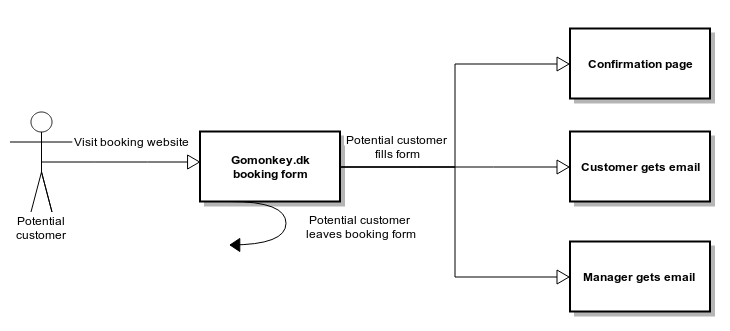
\includegraphics[width=\textwidth]{figures/customer.png}
            \caption{Overview of an initial booking.}
        \label{fig:customer}
\end{figure}

\item[Processing a booking]
The manager reads the booking request email and contacts the customer to provide additional
information if the booking request does not have all the required data. The manager and the 
customer communicate over email until both parties are satisfied with the terms of the booking.
An overview of this can be seen in \autoref{fig:manager}. This manual gathering of additional
booking information can be avoided by building a more complex booking system. After the customer
has supplied all the requested information, the manager then enters the information in Google
Calendar, linking the email with the event. A confirmation email is sent to the customer to
inform him the booking is scheduled.

\begin{figure}[htbp]
    \centering
        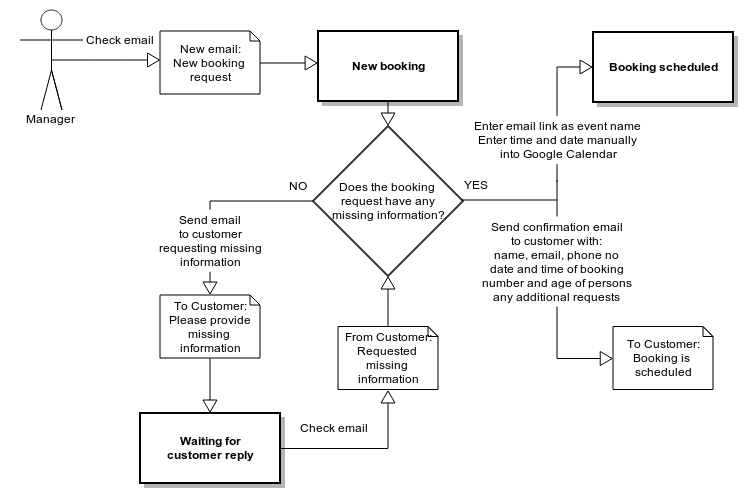
\includegraphics[width=\textwidth]{figures/manager.png}
            \caption{Overview of a booking processing.}
        \label{fig:manager}
\end{figure}

\item[Processing payment]
As seen in \autoref{fig:payment}, the manager is also the one who is processing payments. Every two days,
he logs into his netbank account and associates transactions with their respective bookings in Google Calendar. 
Sometimes customers forget to write their name on their transaction and that causes some distress as the
manager cannot identify the customer. Having to do everything manually leaves room for human error,
a situation which should be avoided. Finally, the manager colors the event associated with the booking
in Google Calendar and changes its description to reflect payment status.

\begin{figure}[htbp]
    \centering
        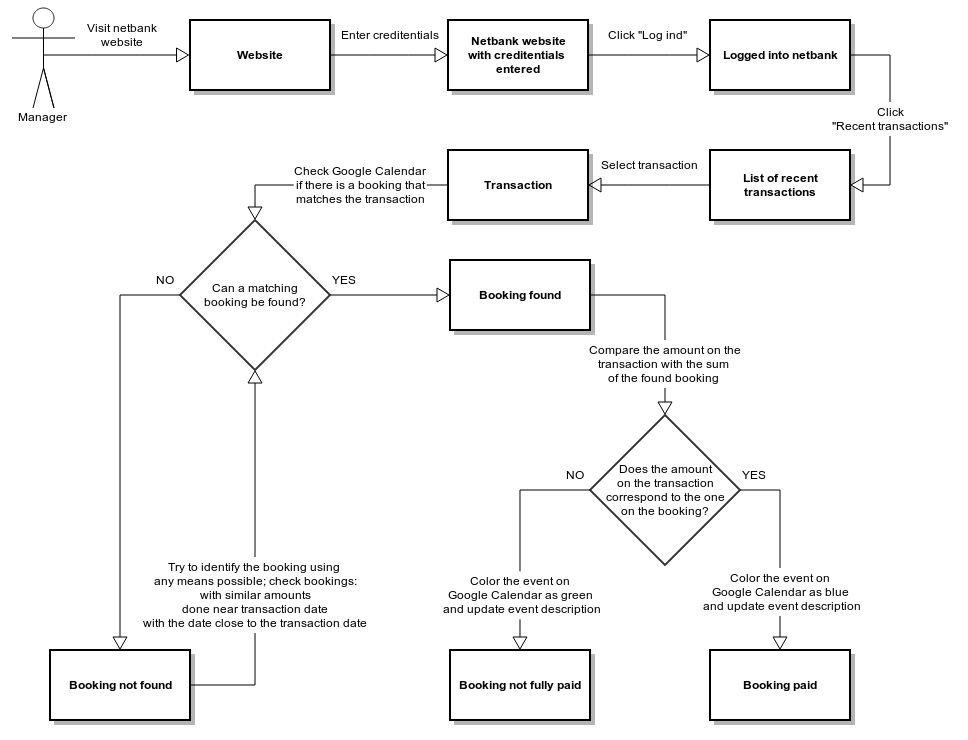
\includegraphics[width=\textwidth]{figures/payment.png}
            \caption{Overview of payment processing.}
        \label{fig:payment}
\end{figure}

\item[Handling booked customers]
On the booked time and date, the customer arrives at \gomonkey{}. He is presented with a security disclaimer
which all the participants from the customers group have to sign. Customers can print the security disclaimer 
at home, but most do not. After taking care of the legal requirements, the instructor present proceeds to
calculate the remaining sum to be paid by the customer, if any. notdone

ref \autoref{fig:handling}

\begin{figure}[htbp]
    \centering
        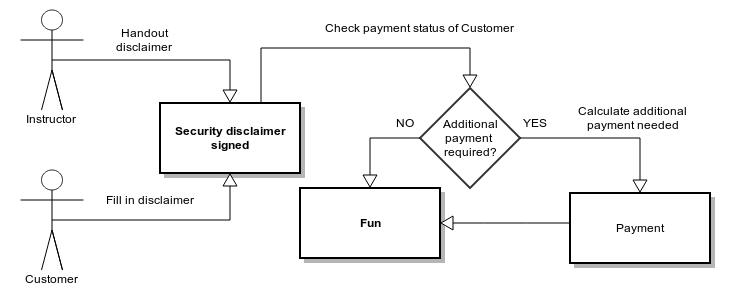
\includegraphics[width=\textwidth]{figures/handling.png}
            \caption{Overview of customer handling}
        \label{fig:handling}
\end{figure}
\end{description}


\subsection{Isolated problems in the current work practices}
The preliminary analysises showed a number of different problems in the current system. 
The design team will refer to these problems when designing the system
to make sure that we are actually solving a problem rather than a symptom
of another problem. The noteable problems that will be solved by the suggested system are listed here.

\begin{itemize}
	\item Customer is disgruntled by the interface.
	\item Conducting complex communication with customer concerning routine questions
	\item Payment is cumbersome and slow.
	\item Entering a booking into the system is cumbersome.
	\item Calculating deficit payment amount at arrival of a booked group.
\end{itemize}

The problems are not in a prioritized order, since all of them have profound
affect on the complete work practices.


\subsection{Searching for a suitable standard system}
A standard system can often lead to a cheap and easy solution to an immediate problem.
We have compiled a list of three very possible
candidates as a supplier for a standard system. 
After deep testing sessions of all systems, we realized that none
of them can solve the problems encountered at \gomonkey{}. The testing
session included creating a free temporary booking system. All systems tend to 
have this feature, so potential customers can evaluate the usefullness prior to 
paying. Attempts were then made to setup the system to support the needs of
\gomonkey{}, and after testing the usefullness of the result, we could conclude
upon the advantages and disadvantages of implementing the system.

\begin{description}
\item[SuperSaaS] is a Joomla! plugin resembling a booking system, that integrates with a 
backend hosted at SuperSaas.

We decided not to use SuperSaaS, since the booking doesn’t support the required 
fields for the booking. A `form' can be attached to a booking after submitting 
initial information (intial information being the date and time of booking, 
name, phone number and email address), and this 
form can include extra information about amount of people in each age group, the
type of customer and food. This information can only be seen after two clicks 
from the calendar overview, thus making it impossible to get a good overview of 
how `available' a time slot is.

Furthermore, it is not possible to calculate a price based on the custom fields 
in the form, and as such, the system cannot ask for a deposit so we will still 
need another payment processor.

\item[onlinebooq.dk] promises a highly customizeable system which can be embedded into
any other existing system.

We did not manage to fit onlinebooq.dk with the requirements of \gomonkey{}.
They support selling 
`services', but unfortunately they only support selling one of each servive.
This can be seen in \autoref{fig:onlinebooq} as the checkbox, next to the 
service in question. This makes it useless for \gomonkey{}, since the price is 
calculated from the amount of people utilizing each service. It does support 
paypal and quickpay, but this doesn't matter if we cannot calculate the price 
correctly.

\begin{figure}[htbp]
    \centering
        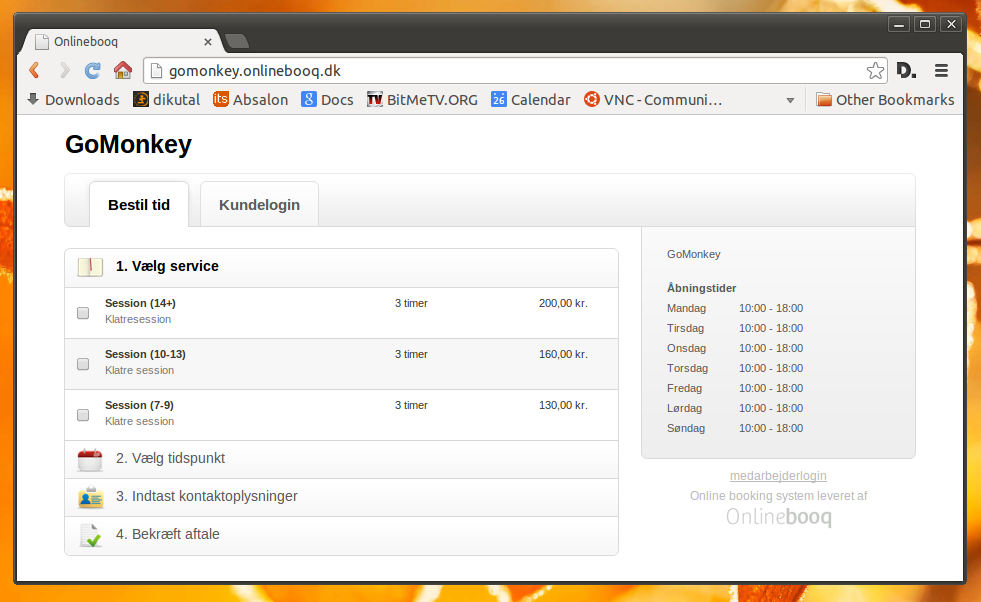
\includegraphics[width=1\textwidth]{figures/onlinebooq.png}
	    \caption{Screenshot from testing onlinebooq.dk.}
        \label{fig:onlinebooq}
\end{figure}
		

\item[Cyberbooking] brands itself as a cheap and simple alternative which runs great 
on mobile devices. 

It turned out to be impossible to fit the services of Cyberbooking with \gomonkey{}. 
Cyberbooking offer two types of 
calendars, one which supports one resource (e.g.\ a hairdresser) who can only
perform one service at a time. The other type supports booking slots on 
predefined events, (e.g.\ a fitness session) and the events are set by the 
company. None of these types can help \gomonkey{} with the booking process,
since the amount of resources aren't limited to one group of customers, and 
the times of bookings are very flexible.
\end{description}

While it is certainly possible to adjust the current work practices to use one of the
mentioned standard systems, this will result in huge changes to the current work
practices, which the design team judge to be very difficult to implement. When weighed
against the alternative of just keeping the current system, we concluded that time would 
be better spend on designing a custom system.


\newpage
\section{Description of the future system}
In the following section we will describe, in detail, how both hardware and
software is expected to be organized and utilized in the future system.

\subsection{Needed software and hardware}
It is a requirement that the main website continues to run on the 
WordPress which is hosted with One.com. This will make
sure that the website maintains it's current, existing Google page-rank. Related 
to this, the system will have to be embedable into WordPress. 

It is necessary to have a server for hosting the new system, with 
access to a database and a webserver. This is not achievable on the server from 
One.com, so another will have to be purchased or rented. It will be sufficient to have 
interfaces to a database and a webserver, but it is optimal to have root acess
to the server.

The server can run any operating system requested by either the developers or
the manager, but picking a free system will avoid the costs of licenses for 
proprietary systems.

Additionally, there will still be parts of the original system which remain. 
The scheduling and journaling of staff will still be hosted in the company's 
Google Drive. 

\subsection{Components, functions and interface}
The new booking system contains 5 components. The components will be described 
with the necessary figures from the produced mockup. The function of the 
components will be explained and in a later section it will become apparent
how the mockup actually solves the encountered problems. The components are:

\begin{itemize}
\item Customers booking process
\item Customers payment and overview of booking
\item Managers overview of incoming bookings
\item Managers processing of an incoming booking
\item Instructors overview of todays bookings
\end{itemize}

The first page supporting the \textbf{customers booking process} can be seen in \autoref{fig:bookinitial}. The booking
form incorporates many of the original features and functions of the existing 
\gomonkey booking form along with some new fields further supporting the envisioned work practices. 
The user is expected to input values for a number of 
different fields required for a booking. The specific fields seen in the figure
are the necessary fields required to support the following process.

The price calculator is a part of the booking form, that provides 
a running total of the cost of the booking as well as any deposit, if the cost
of the booking is large enough. Also, A Frequently Asked Questions section is 
located directly in the booking form, for easy viewing during booking.

\begin{figure}[htbp]
    \centering
        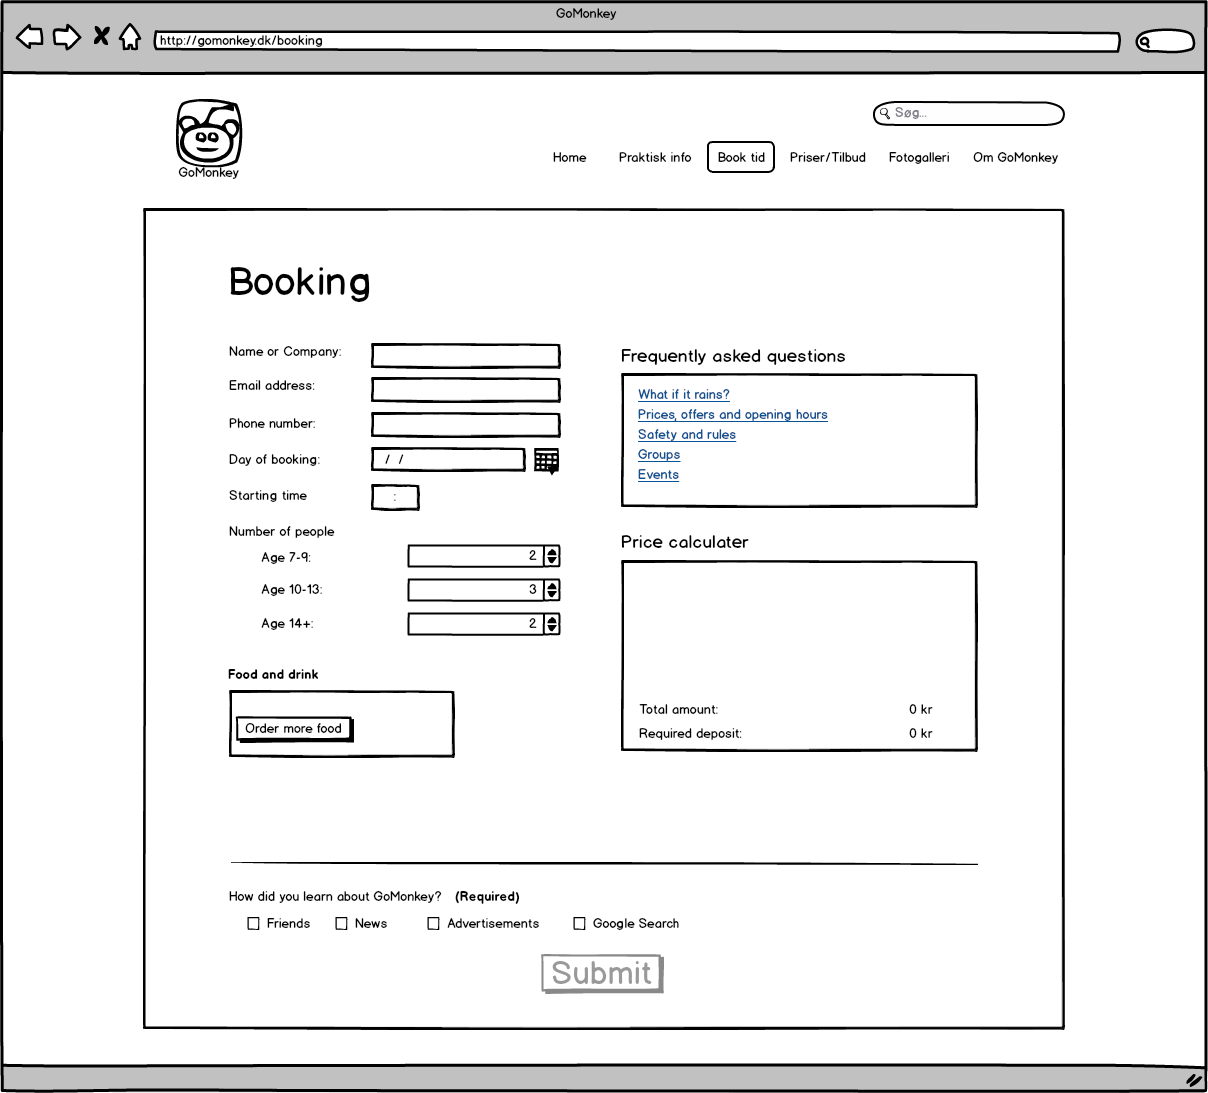
\includegraphics[width=.6\textwidth]{figures/mockup/booking_initial.png}
	    \caption{The bare booking form which the customers will find on the WordPress website.}
        \label{fig:bookinitial}
\end{figure}



An example of a filled booking page can be seen in \autoref{fig:bookfilled}. 
The system will ensure that all data is entered in a valid way, such that the form
will not allow an invalid booking. This could be a booking with zero
participants, or a date that has already passed. The
'Submit' button will prepare the booking for a final view for the customer to 
confirm that the information are indeed correct, or to be able to fix any errors 
not caught by the input validation in the form.

\begin{figure}[htbp]
    \centering
        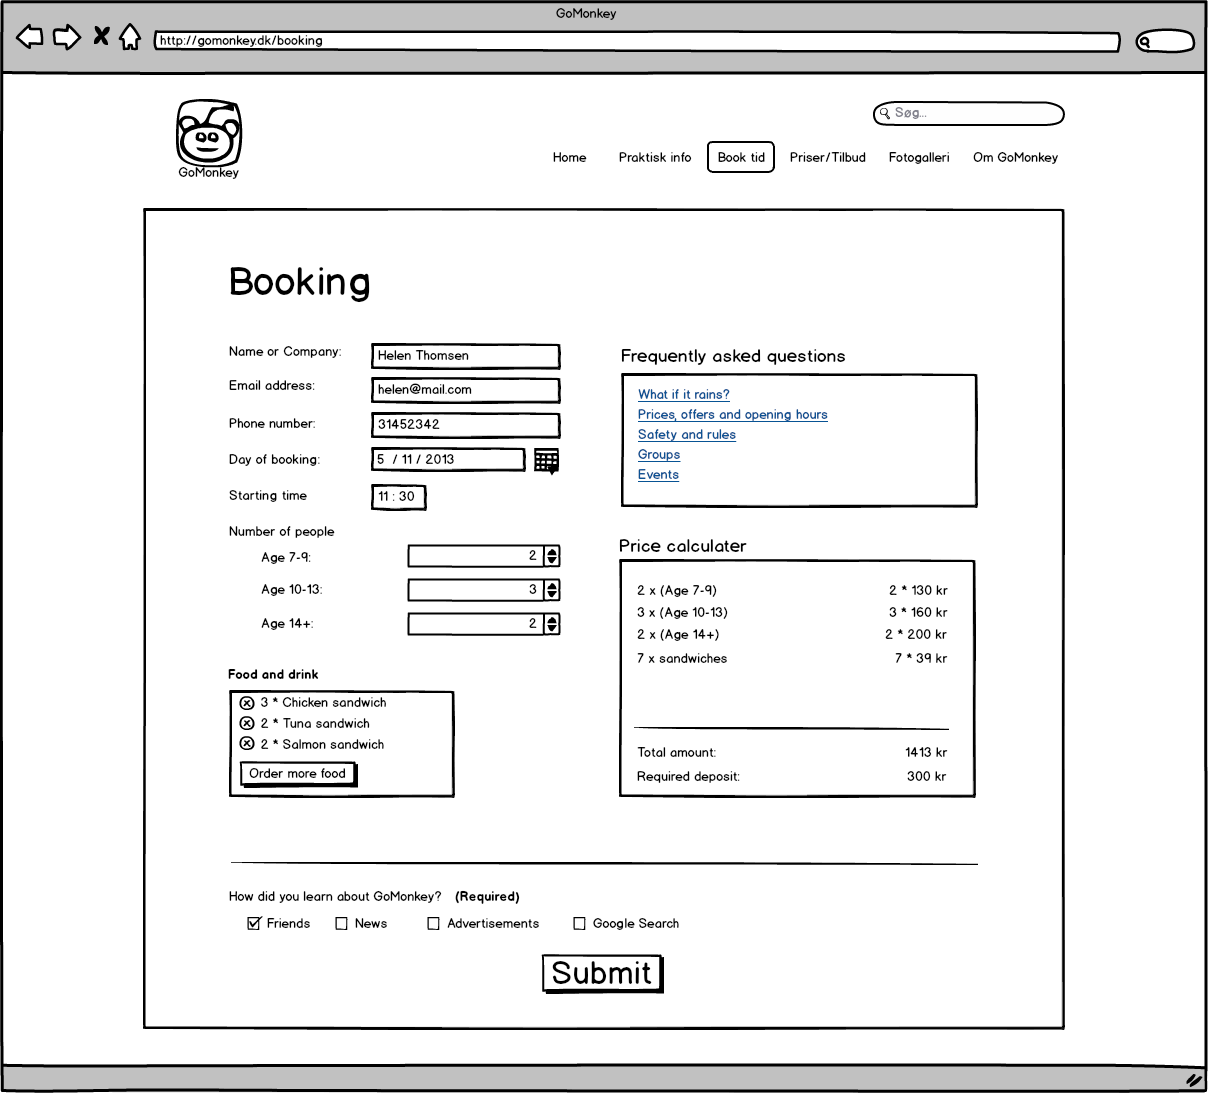
\includegraphics[width=.6\textwidth]{figures/mockup/booking_filled.png}
	    \caption{The booking form is filled and ready to be submitted.}
        \label{fig:bookfilled}
\end{figure}



The reached page displays all the entered information in much the same structure as 
the booking input page, but 
without any editable fields. This can be seen on \autoref{fig:bookconfirm}. If the 
customer is not satisfied with the entered data, it is possible to return to the 
previous booking form to correct any errors by clicking 'Back' in the bottom of the page. 

\begin{figure}[htbp]
    \centering
        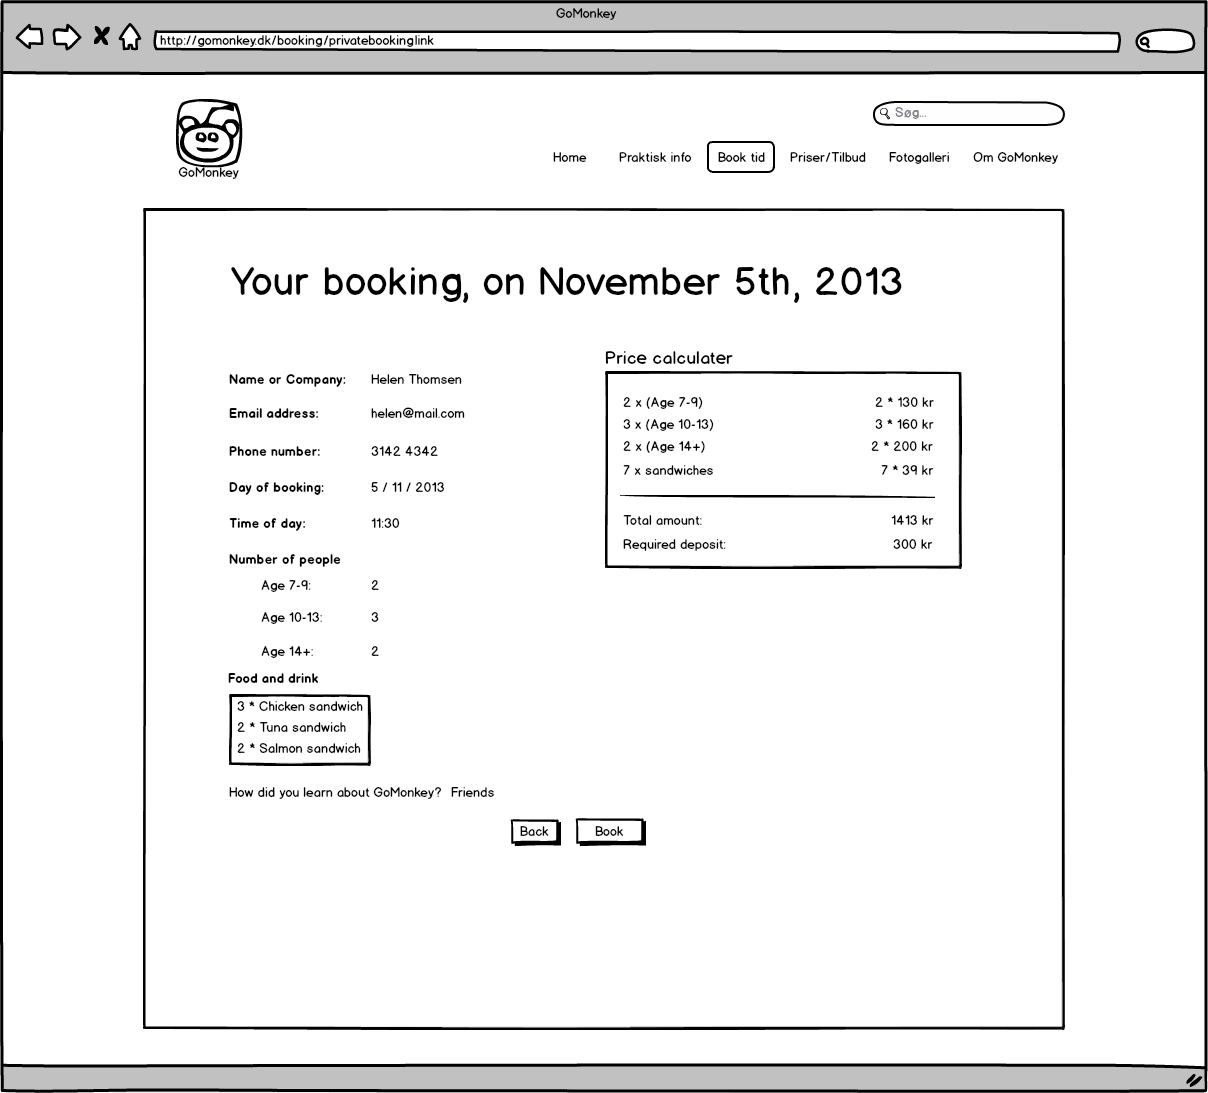
\includegraphics[width=.6\textwidth]{figures/mockup/booking_confirmation.png}
	    \caption{The booking form is submitted and the customer can view the entered information before finally booking.}
        \label{fig:bookconfirm}
\end{figure}



If the user agrees to the entered information, the
user can click 'Book' and the booking will be sent while the user is presented
with a modal popup that informs the user that the booking will need to be confirmed,
and that there might be a required deposit. This can be seen on 
\autoref{fig:bookconfirmpressed}.

\begin{figure}[htbp]
    \centering
        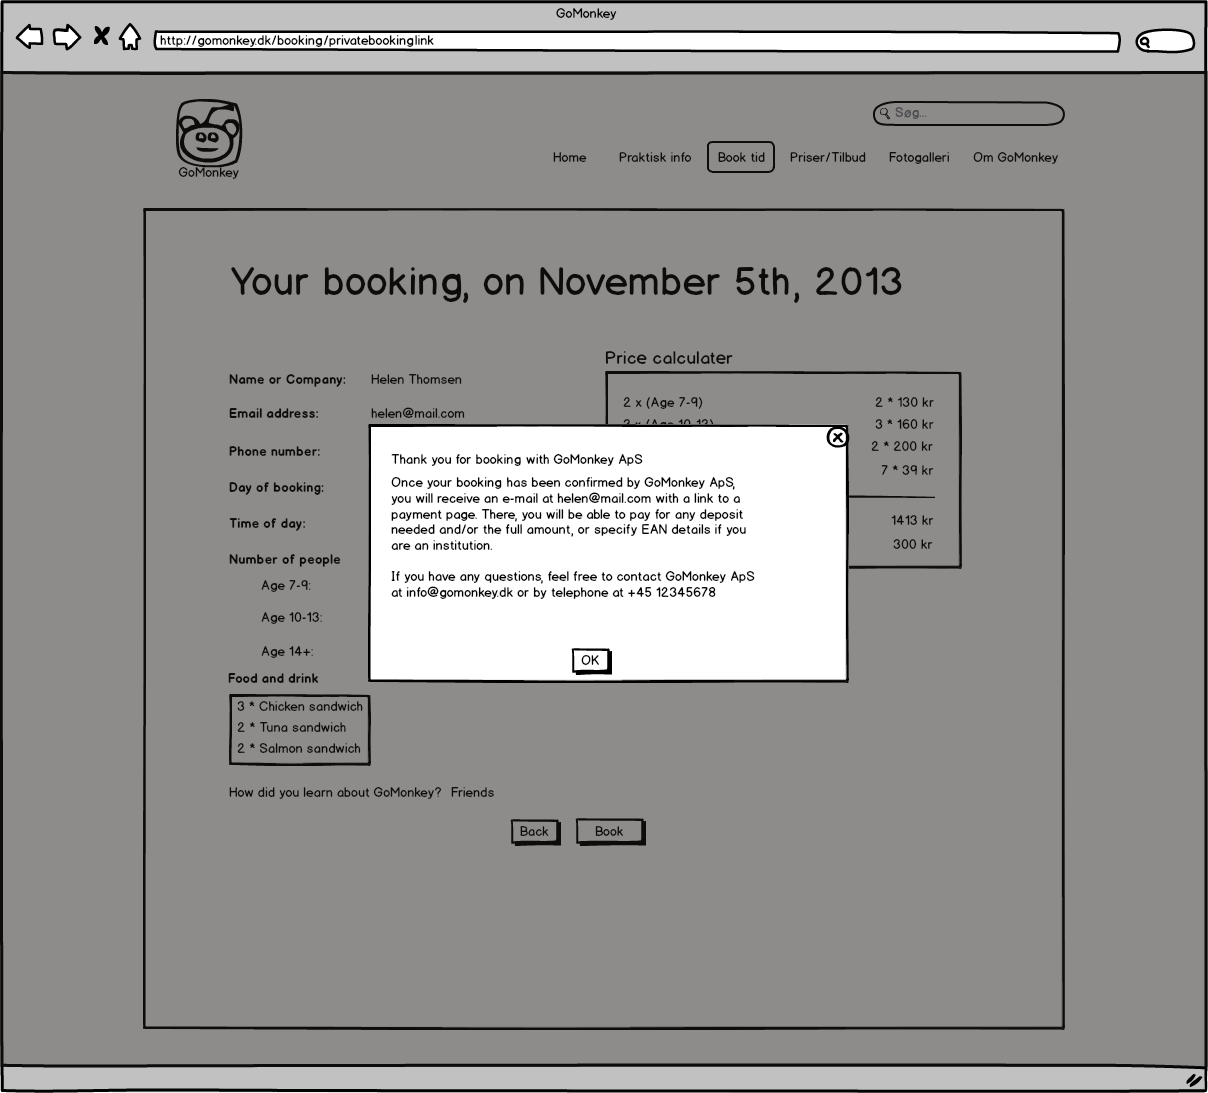
\includegraphics[width=.6\textwidth]{figures/mockup/booking_confirmation_bookpressed.png}
	    \caption{The booking form is submitted and the customer is informed about the following process.}
        \label{fig:bookconfirmpressed}
\end{figure}

\FloatBarrier
\newpage

The page supporting the \textbf{customers payment and overview of the booking} 
looks quite similar to the booking form, but the 
user cannot make any changes to the booking. In addition to a list of all of 
the things the user could see in the booking form, the user can also see 
whether \gomonkey{} has confirmed the booking or not. The case where is it not confirmed can be seen on \autoref{fig:bookstatus1}

\begin{figure}[htbp]
    \centering
        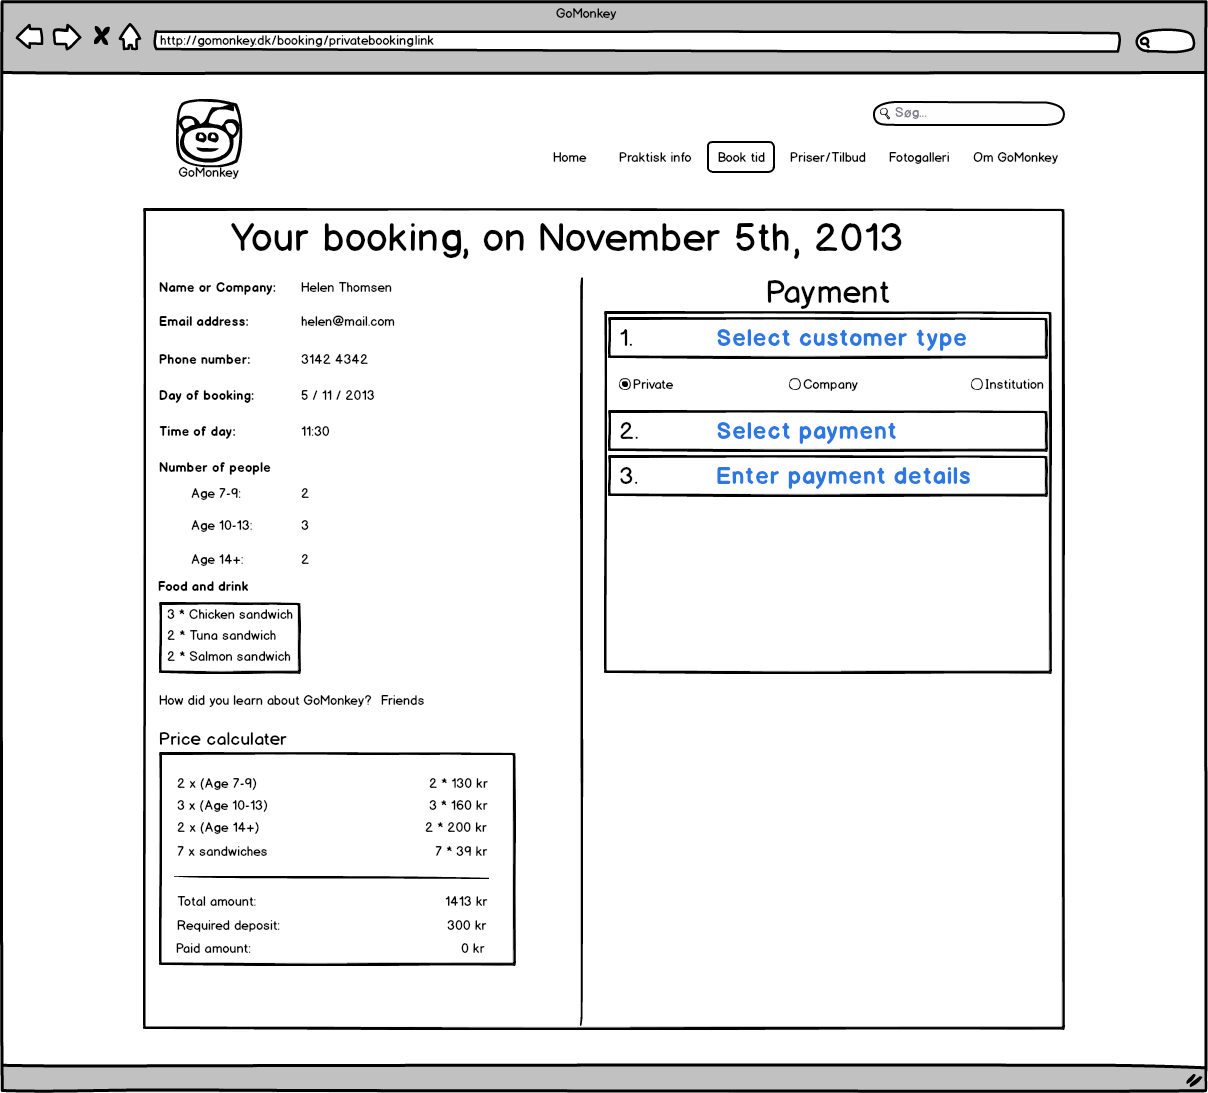
\includegraphics[width=.6\textwidth]{figures/mockup/booking_payment_1.png}
	    \caption{The customer can see the booking, but can't pay until the date and time has been confirmed.}
        \label{fig:bookstatus1}
\end{figure}

An unconfirmed booking can not yet be paid for in any way. However, once a 
booking is confirmed by \gomonkey{} the payment options appear, as in 
\autoref{fig:bookstatus2}. Payment occurs 
by clicking on either a ‘Pay Deposit’ button, or a ‘Pay full amount’ button. 
For institutions, there is also a ‘Confirm payment via EAN’ button, which 
allows the user to enter EAN-related details instead.

\begin{figure}[htbp]
    \centering
        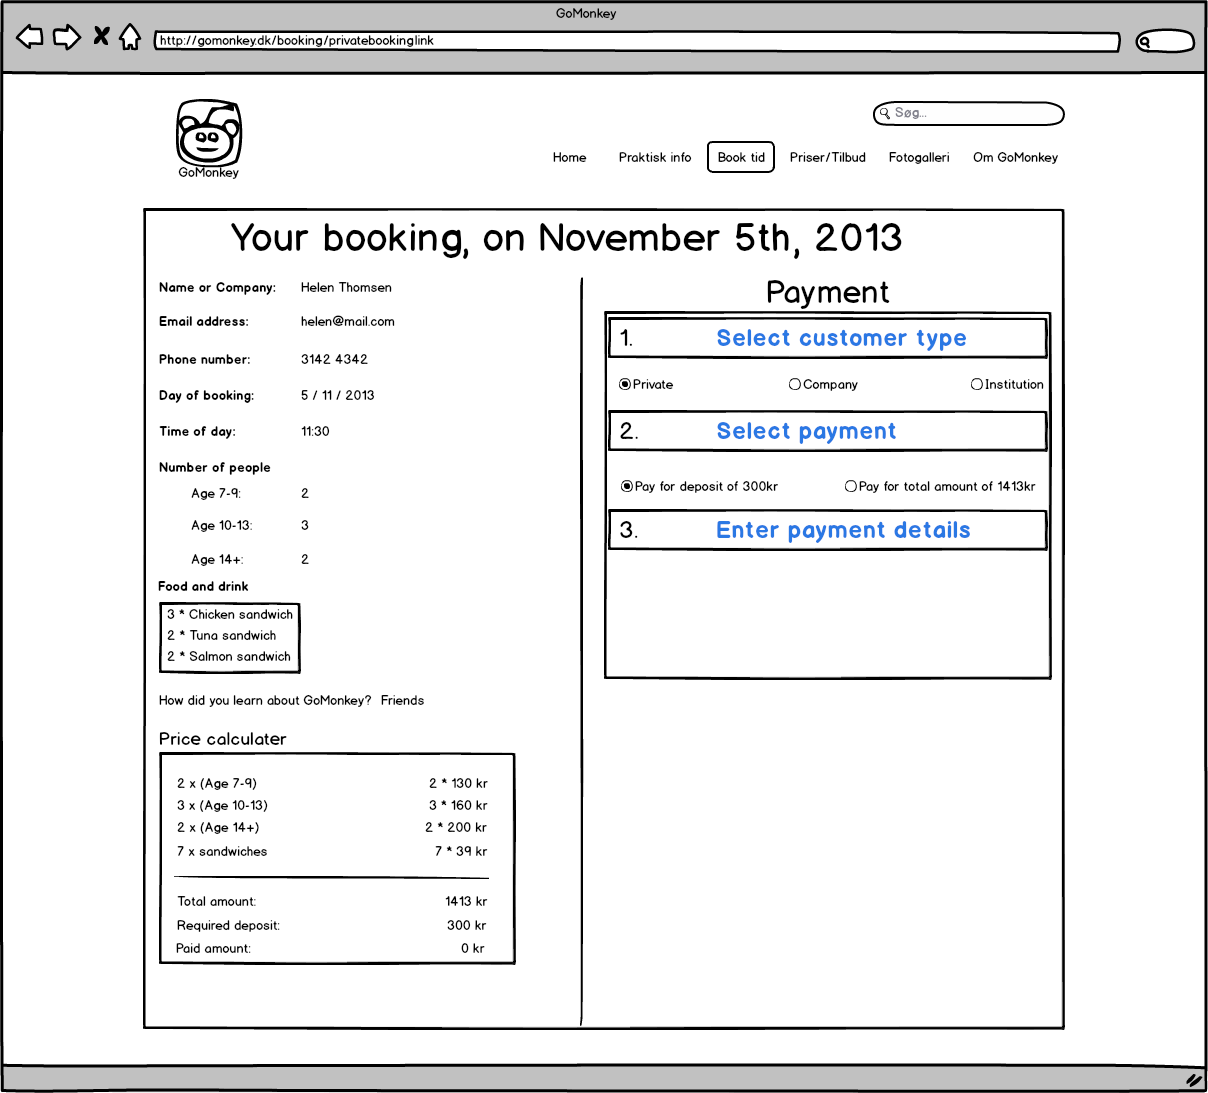
\includegraphics[width=.6\textwidth]{figures/mockup/booking_payment_2.png}
	    \caption{The customer is now able to select the desired amount to be paid, prior to visiting the park.}
        \label{fig:bookstatus2}
\end{figure}

Finally, when an amount has been selected, is is possible to select a preferred
payment processor, as in \autoref{fig:bookstatus3}. This is important, since 
instant online transactions are very
critical to the function of the system.

\begin{figure}[htbp]
    \centering
        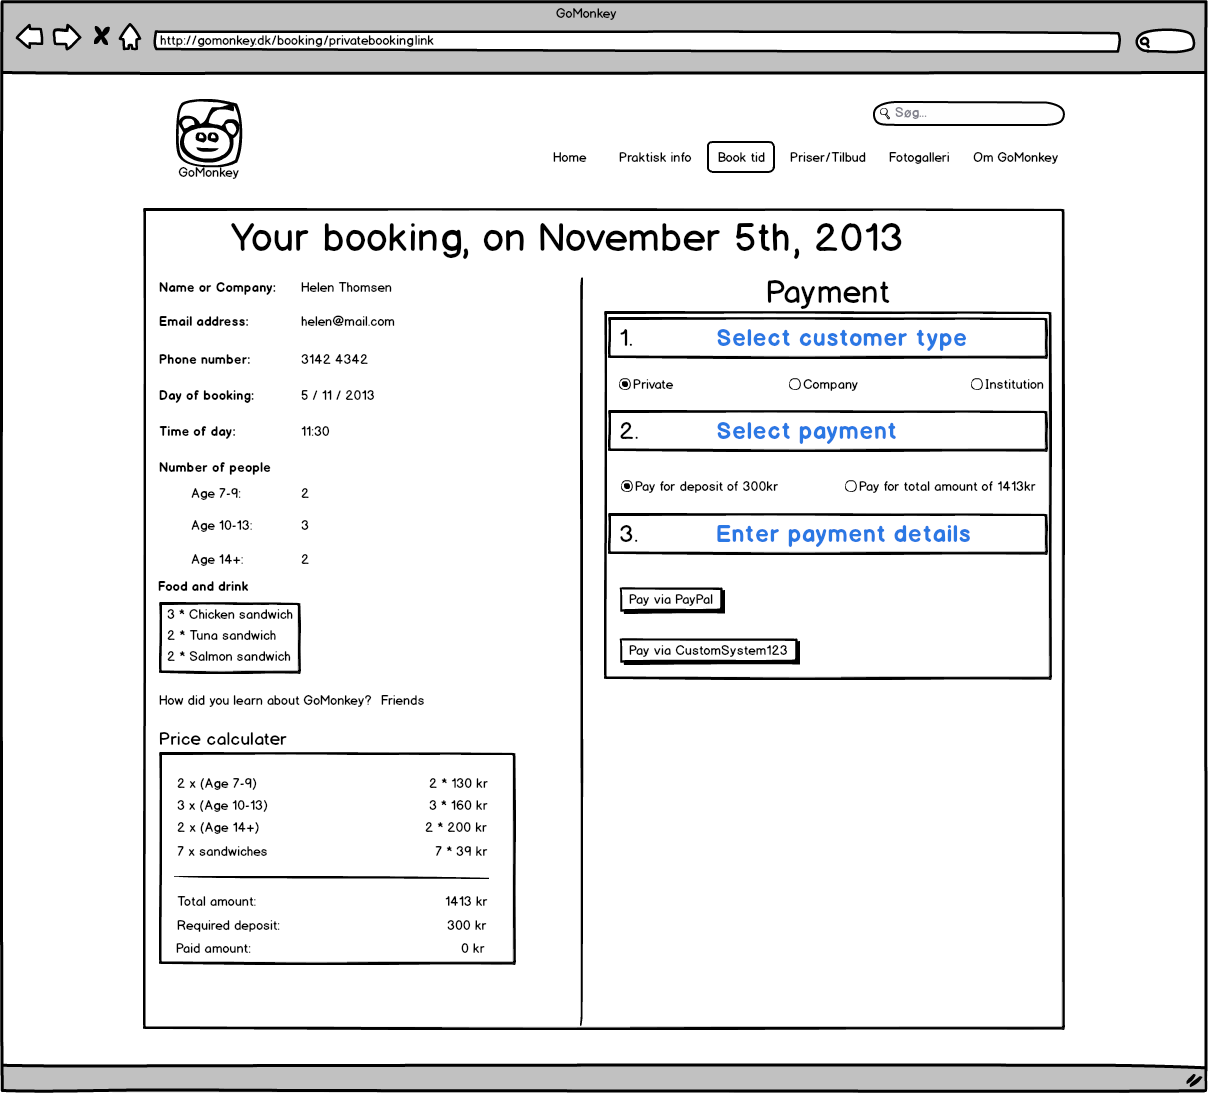
\includegraphics[width=.6\textwidth]{figures/mockup/booking_payment_3.png}
	    \caption{Finally, the customer can select a preferred payment processor and pay instantly.}
        \label{fig:bookstatus3}
\end{figure}

\FloatBarrier
\newpage

The page supporting \textbf{managers overview of incoming bookings} displays a list of bookings which require an 
action from the manager, and can be seen in \autoref{fig:adminoverview}. The 
date, time and amount of people is shown for a quick overview, and each booking can be viewed with the following 
component.

\begin{figure}[htbp]
    \centering
        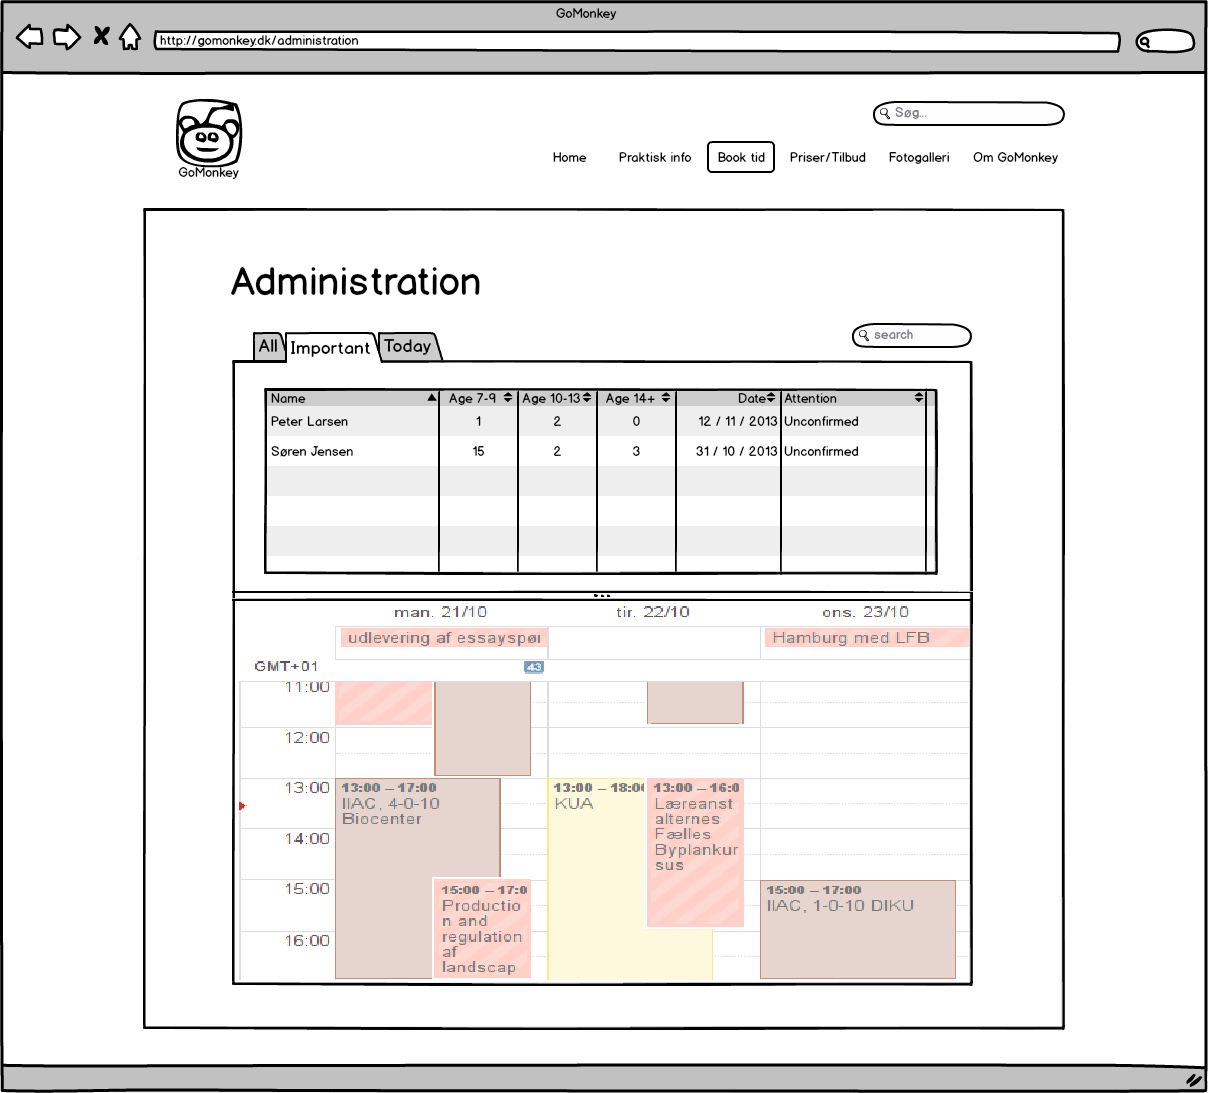
\includegraphics[width=.6\textwidth]{figures/mockup/overview_important.png}
	    \caption{The manager has a good overview of the incoming bookings which requires a reaction.}
        \label{fig:adminoverview}
\end{figure}

\FloatBarrier
\newpage


The page supporting the \textbf{managers processing of an incoming booking} shows the entered data of
a single booking and allows the
\gomonkey{} manager to either confirm a booking or decline it, based on the 
calendar overview presented next to the confirmation box. This can be seen in
\autoref{fig:admin}. 

\begin{figure}[htbp]
    \centering
        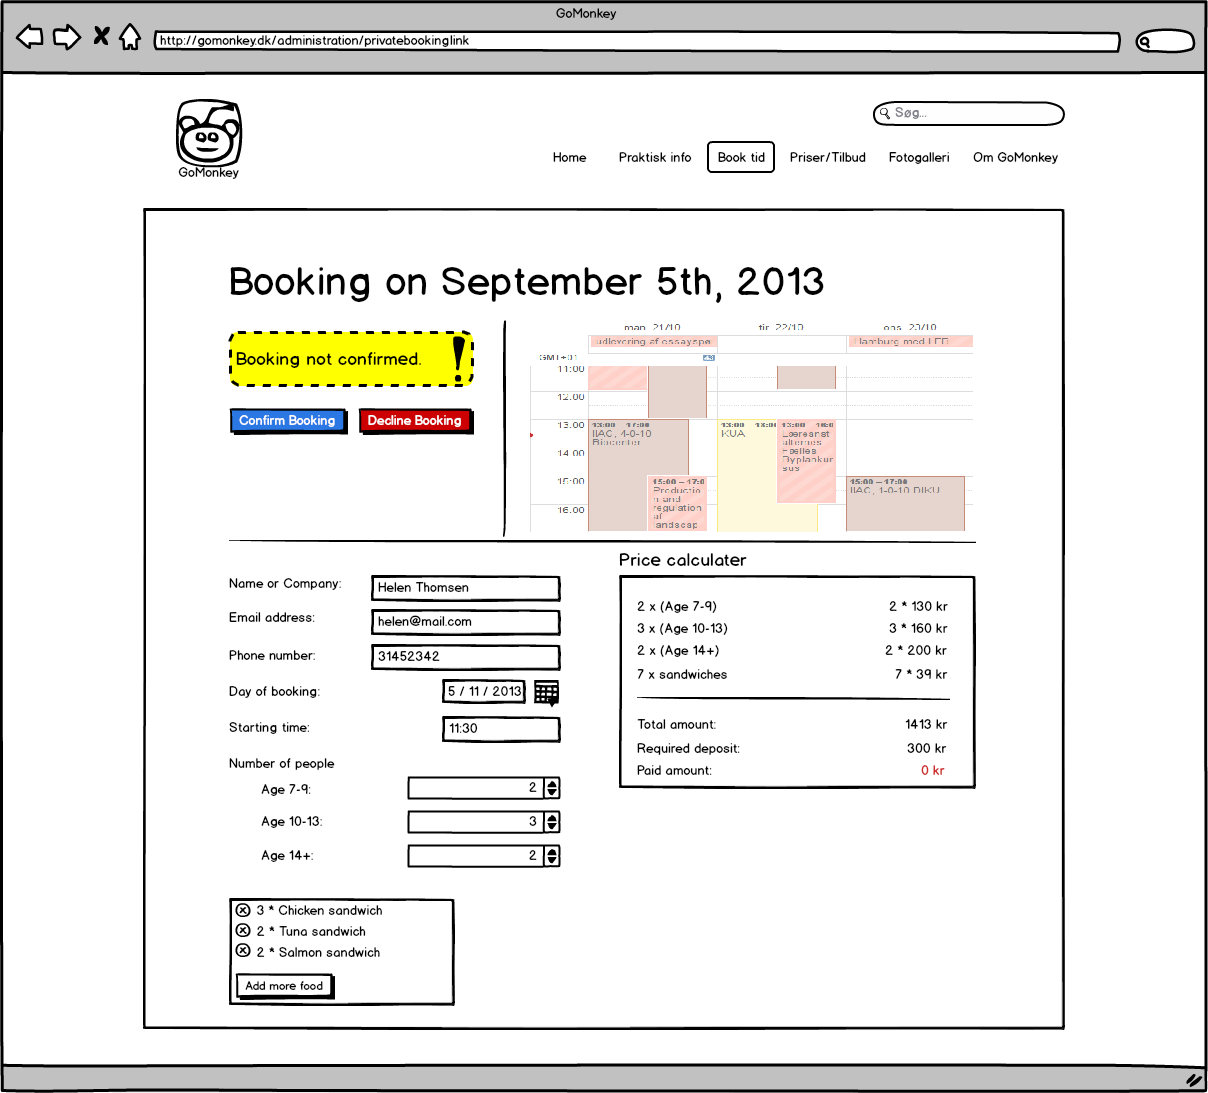
\includegraphics[width=.6\textwidth]{figures/mockup/admin_booking.png}
	    \caption{The manager can view the booking and see the calendar dates surrounding the booking.}
        \label{fig:admin}
\end{figure}

If the manager accepts a booking, an e-mail will be sent to the user notifying 
them of this, and the user-viewable booking status page will reflect that the 
booking has been accepted. The booking is now open for the user to pay 
deposit/full amount. This can be seen in \autoref{fig:adminconfirmed}.

\begin{figure}[htbp]
    \centering
        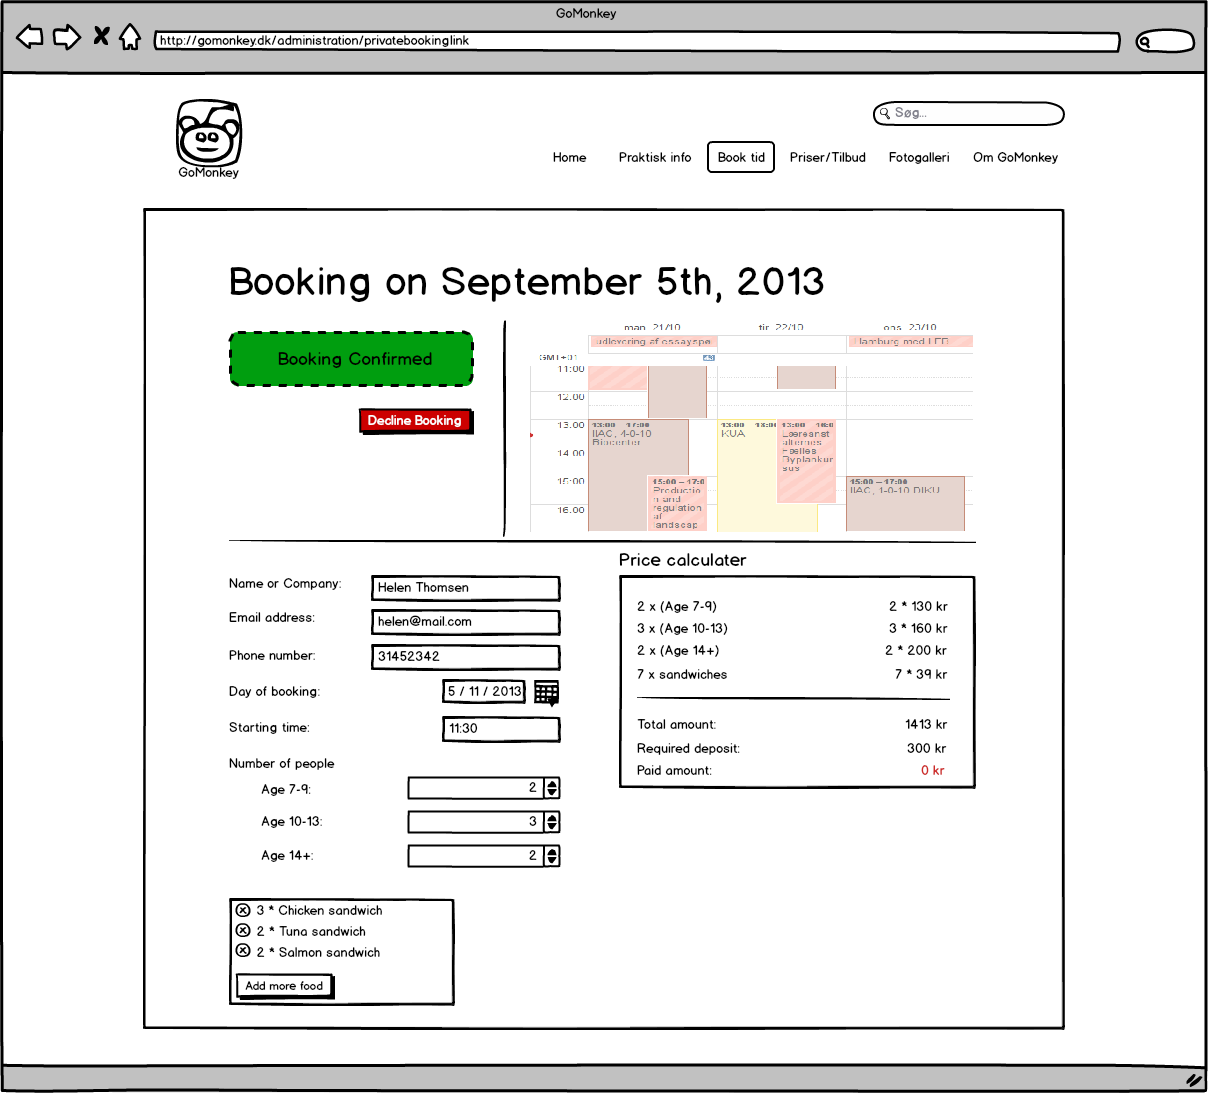
\includegraphics[width=.6\textwidth]{figures/mockup/admin_booking_confirmed.png}
	    \caption{The manager has confirmed and the customer can now pay for the session.}
        \label{fig:adminconfirmed}
\end{figure}

If the manager declines a booking, an e-mail will be sent to the user notifying 
them of this, and the user-viewable booking status page will reflect that the 
booking has been declined. The manager can supply a reason at the time of 
declining, with either a standard response, or a manual response with a
suggested alternative time and date. This can be seen in \autoref{fig:admindecline}

\begin{figure}[htbp]
    \centering
        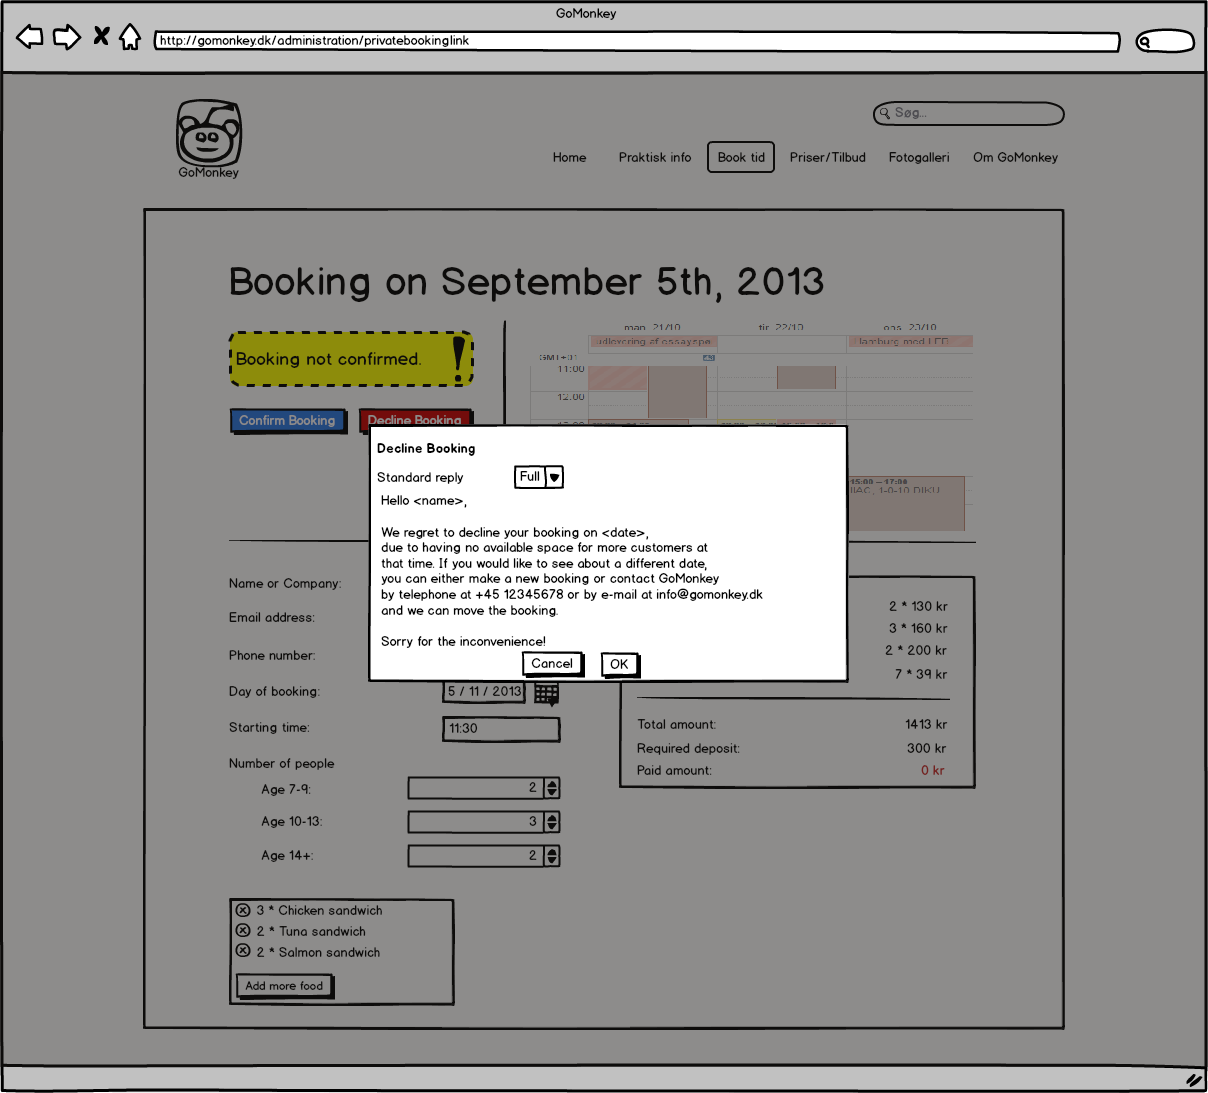
\includegraphics[width=.6\textwidth]{figures/mockup/admin_booking_decline.png}
	    \caption{The manager can decline the booking with a message describing why he had to decline, or attach a custom message.}
        \label{fig:admindecline}
\end{figure}

\FloatBarrier
\newpage

The final component is the \textbf{instructors overview of todays bookings} and can be seen in
\autoref{fig:overviewtoday}. This is intended for 
the instructor to get a quick overview of how many people are coming on the 
day, when they will come, and how much they will need to pay, and whether
they ordered something extra. This will help the instructor handling booked 
groups. Especially if there is a booking for a big group, the instructor will
know not to take big groups just prior to having the booked group arrive.

\begin{figure}[htbp]
    \centering
        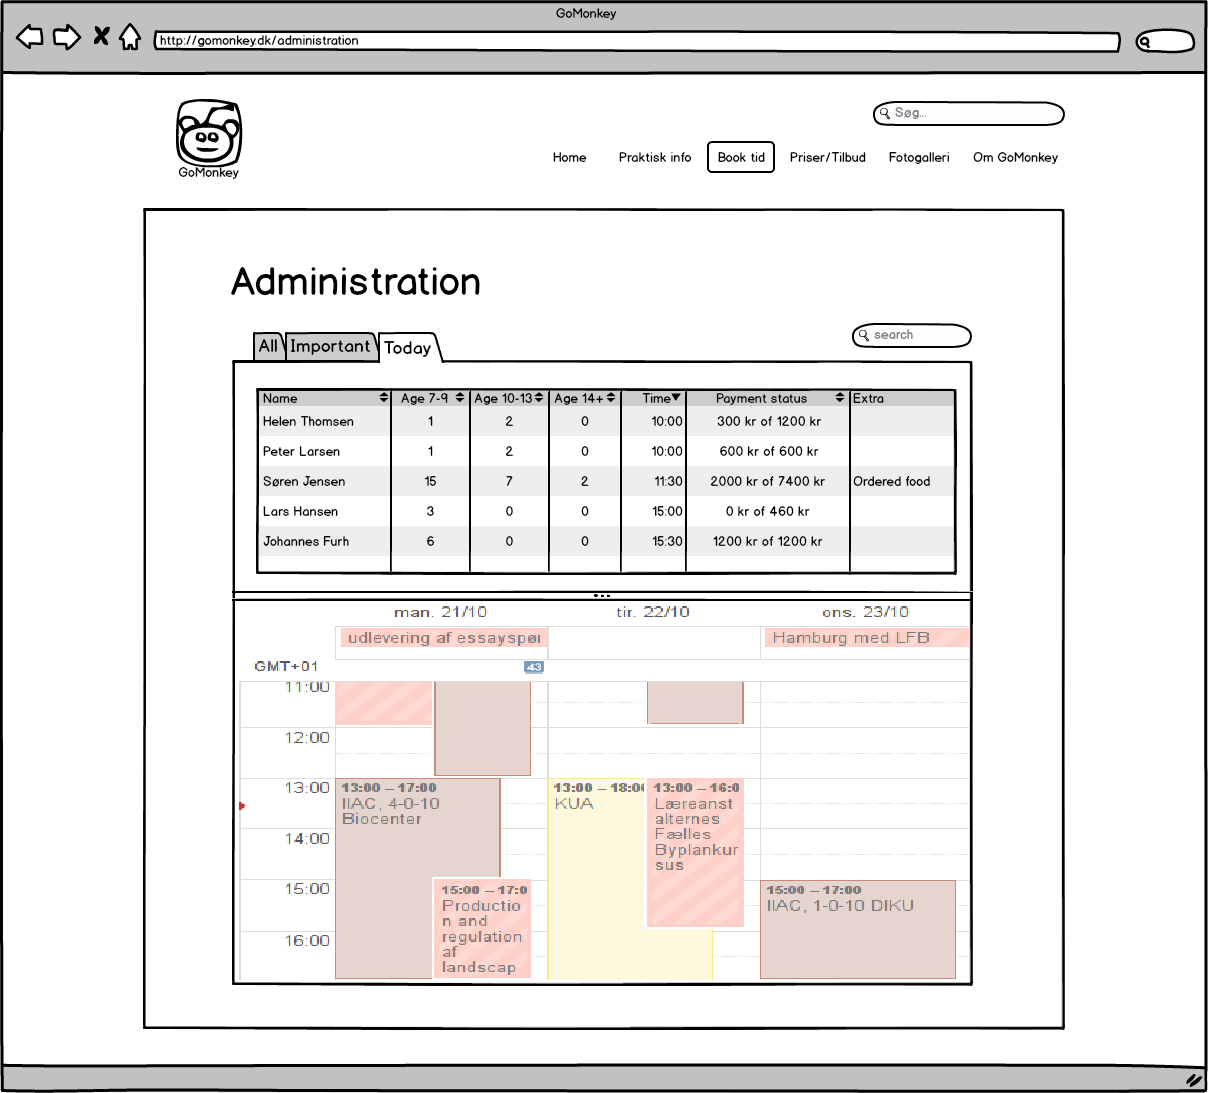
\includegraphics[width=.6\textwidth]{figures/mockup/overview_today.png}
	    \caption{The instructor can easily see what times there will be incoming groups.}
        \label{fig:overviewtoday}
\end{figure}


\subsection{Envisioned future work organization}
The future work organization suggested is very simliar to the current 
work organization. Currently, the manager and the owner are always the same 
persion. The owner often also takes the role of an instructor, to reduce the 
hourly wages needed to be paid. 

The tasks of the owner is to evolve the business in a direction that hopefully 
advances toward achieving the business strategy. We define the tasks of the 
manager to be the everyday processes required to keep the business running. 

The last group in the work organization is the instructors, whose only task is to
receive customers, booked or not, instruct them on the courses and taking 
correct payment from the customers.

In the old system, part of the work practice relating to checking payments 
was very difficult to distribute to another employee due to the requirement
of access to the owners personal bank account login solution. The new system
does not entail that restriction, and so it is far easier to distribute managerial
tasks to other employees, should the owner desire to do so.

\subsection{Specific qualifications required in using the new system}
We assume that the instructors are familiar with using a calendar overview from 
the current system. They will 
still have to be shown how to navigate to the view of the bookings on the 
current day, and how to interpret the information which is now visible.

The manager and owner need deep knowledge of the system, and how bookings are to 
be managed and handled. It will be necessary to introduce the system to a level
where the manager and owner feels comfortable using the system, and teaching 
the instructors how they should use the system.

The booking form is tailored to help a customer perform the desired booking with 
as few errors as possible. We assume that the customer uses the internet on a 
weekly basis. The ease of using the booking formula was a 
requirement for designing the booking form, so the necessary information and
guidance is available to the customer to avoid any frustration that confusion
could result in.

\subsection{Advantages and disadvantages of the future system}
In this section we will describe what advantages the vision will bring to 
\gomonkey, in relation to the current situation. This will help value the advantages against the disadvantages and
price of the system. With this information it will be possible to make an informed
choice on whether to implement the system, or not.

\subsubsection{Business- and IT strategies}
Here we describe how the proposed system helps advance the company towards their 
business strategy, which was defined earlier in the design report. 

\begin{description}
\item[Become a self-sustainable climbing company with customers on a daily basis]
To become self-sustainable company, it will be necessary to have enough profit
to not have to sort to 'solving emergencies'. The owner will have to be able 
to leave most of the work to employees, without taking a significan hit in 
profit. This system puts the booking in a very defined process, and thus 
simplifies it a lot. It becomes a lot simpler, so the manager will,
with the correct employee, be able to pass on the task, to focus on other parts
of the company.

Economically, it is hard to define an absolute increase in profit, and the 
result may only be achieved some time after deploymen. And, since 
\gomonkey{} is such a new business, it is going to be very difficult to account
the measured differences to the implementation of the system, since we know 
nothing of the 'average' income.

\item[Minimize time requirements pr.\ booking/customer]
The system will support most
of the situations which currently require a lot of correspondance between the 
manager himself, and the customer. There is no need to check the bank account,
which is a time consuming task, and very prone to errors. The requirement for 
intervention from the manager is drastically reduced in the new system, because
many of the manual tasks are automated.

\item[Minimize staff requirements to keep costs low]
The system does little to actually minimize staff, but indirectly, the manager
can, with more time at hand, do more work to coordinate staff in a more 
economically viable manner. Further, when the company gets more customers,
there will be less situations where it is necessary to staff a situation where
there is only a low income, which has occurred and often resulted in a declination
of the booking.

\item[Increase sales (such as selling food and drinks)]
The system supports selling more than just the single service of a visit to a climbing park. It is a lot
easier for customers to buy additional services, such as food and drinks, due to 
the direct support for this in the new system, compared to the complicated 
process of offering, accepting and ordering food.
\end{description}

\subsubsection{Groups of staff and their relations}
This section describes how the new system will help the staff do their 
job, and what drawbacks there may be, in relation to the old system.

\begin{description}
\item[Advantages]
The new system will be an
advantage for the instructor at work to have a more of the needed information
at hand, such as decifit price and amount and age of the coming customers. 
This will make for a less error prone handling of customers. The 
decifit price will be available to the instructor, instead of having to 
calculate the price manually. Further, the situation where a customer paid on 
the day and thus the instructor can't see the paid amount will completely be 
avoided, since the system is built to only support payment processors with 
instant transaction confirmations.

\item[Disadvantages]
The manager is very invested in the system, and will want the employees to 
use the system as soon as possible. The instructors may be less ready for the change and may
oppose spending time learning a new system. This can result in friction between
the two groups and can potentially result in a very uncomfortable work 
environment. 
\end{description}

\subsubsection{Customers}
This section describes how the results of implementing the coherent vision will 
effect the user experience of customers in both positive and negative 
directions.

\begin{description}
\item[Advantages]
Previously, a lot of communication was very cumbersome, but 
with the new system, much of the communication is no longer needed. The 
ordering of food and exchange of necessary information is now handled by the 
new booking form, which will in turn be a more efficient work practice.

The reduced amount of cumbersome communication and easily understandable system
will also be partly visible for the customer, since the company will seem more
professional.

\item[Disadvantages]
The reduced amount of personal communication may lead the the booking process having
a less personal feeling for the customer. Knowing that you are writing with
another human being that actually caters for your specific needs is a very 
powerful effect, which will not be as utilized in the future system. 
\end{description}

\newpage
\section{Finances and costs}
We suggest here an estimate of how much we believe the system will cost. This
is based on the design teams knowledge of pricing IT systems and their 
prior experiences with such projects. 

To build the system it is necessary to hire a programmer and a graphics artist.
It is also necessary to have a server running permanently, hosting the system. 
The prices of those are estimated to be:

\begin{itemize}
\item Front-end programmer, \textbf{500DKK/hour}
\item Graphics artist, \textbf{500DKK/hour}
\item Server hosting, \textbf{100DKK/month}
\end{itemize}

We estimate the following time requirements:

\begin{itemize}
	\item 30 hours of a programmer, to turn mockups into an initial prototype and integrate with the existing site.
	\item 10 hours of a graphics artist in total, to create art assets for the website.
\end{itemize}

This brings the total cost of such a venture to \textbf{20.000DKK} plus, for the 
development of the system. During the development phase, the server hosting
fees will also have to be paid, and is added over the course of development.

After the development period, the server hosting fee will still have to be paid
for as long as the system must remain online and useable. 

It is necessary to annual maintenace on the system, which includes security updates
and server maintenance. We estimate that this will take approximately 10 hours per year, 
and will amount to \textbf{5.000DKK/year}.

\newpage
\section{Implementation strategy and plan}
The following section is a suggested step-by-step guide on how to develop, 
deploy and implement the new system into the current work organization. We 
will refer to a project responsible, which may very well be the owner and 
manager of \gomonkey{}.

\subsection{Technical implementation}
The project responsible will have to contract an IT solutions supplier who 
master the required knowledge of building the suggested system. They need
a graphics artist and a programmer with knowledge of how to build a system
which is embedable into a WordPress installation. The developing entity
should read the design report prior to agreeing to the contract and
price. 

The projects responsible and the developers will have to agree on what server
hosting supplier is chosen for the system, since \gomonkey{} will have to maintain
contact with the supplier, even after the system has been developed. The 
developers should also have an effect on what supplier is chosen, to ensure that
they have the necessary access and tools to perform the development of the
system. Possible suppliers could be either german Hetzner, danish
Rackspace or Amazon.

During the development phase, it should be possible for the project responsible
to monitor the progression of the system, to ensure that misconceptions are 
caught as early as possible.This will help keep the deliverables on track with
the set time schedule. If this fails, a fair agreement on who pays for the 
extra work should be worked out in the initial contract with the developers.

Once the system has been developed by the developing entity, the manager should meet up with 
them, and they should perform thorough manual testing and play scenarios, 
attempting to visualize how the system will work with a customers. The
developers have probably built even more webpages or some other way to view 
log files and other monitoring tools, which should also be shown to the manager. 
This will help the manager perform simple surveillence of the systems health.

Finally, the developers should deliver a thorough documentation of the 
delivered system which can be passed on to anyone who should be required to 
perform maintenance or further development on the system. This will drastically
reduce the price of such future interventions related to the IT system itself.

\subsection{Organizational implementation}
A new IT system will affect the whole 
organization, and thus it is necessary to prepare for the changes, and be very
vigilant when adapting the company to a new system. 

The requirement for organizational preparation arises after the system has been
put into production. It is necessary for the employees to be prepared for
switching to a new system. This can be done by informing the employees about how the project is coming along, over 
the course of the development. This will give the employees a chance to accept 
the changes over a longer period, 
giving the idea time to 'sprout and bloom' before they will need to use the 
system. This will increase the readiness for change.

When the system is finished, and ready to be used, the manager should perform
a training session with the employees. This can be done with every single
instructor, or by inviting all of them for a single session, depending on what
the manager feels most comfortable with. The session should include showing most of 
the system, even the parts they will not use themself. Performing scenarios
with the instructors, using the new system will further help the understanding
of their new role. This session will give the instructors the final idea
of why the system is good for the company, and equips them for guiding the 
customers in a better way, since they are aware of the whole user experience.

\newpage
